% !TEX encoding = UTF-8 Unicode
% !TEX root = ../report.tex
% 

\section{Construcción de la ontología}

\begin{figure}[h!]
  \makebox[\textwidth][c]{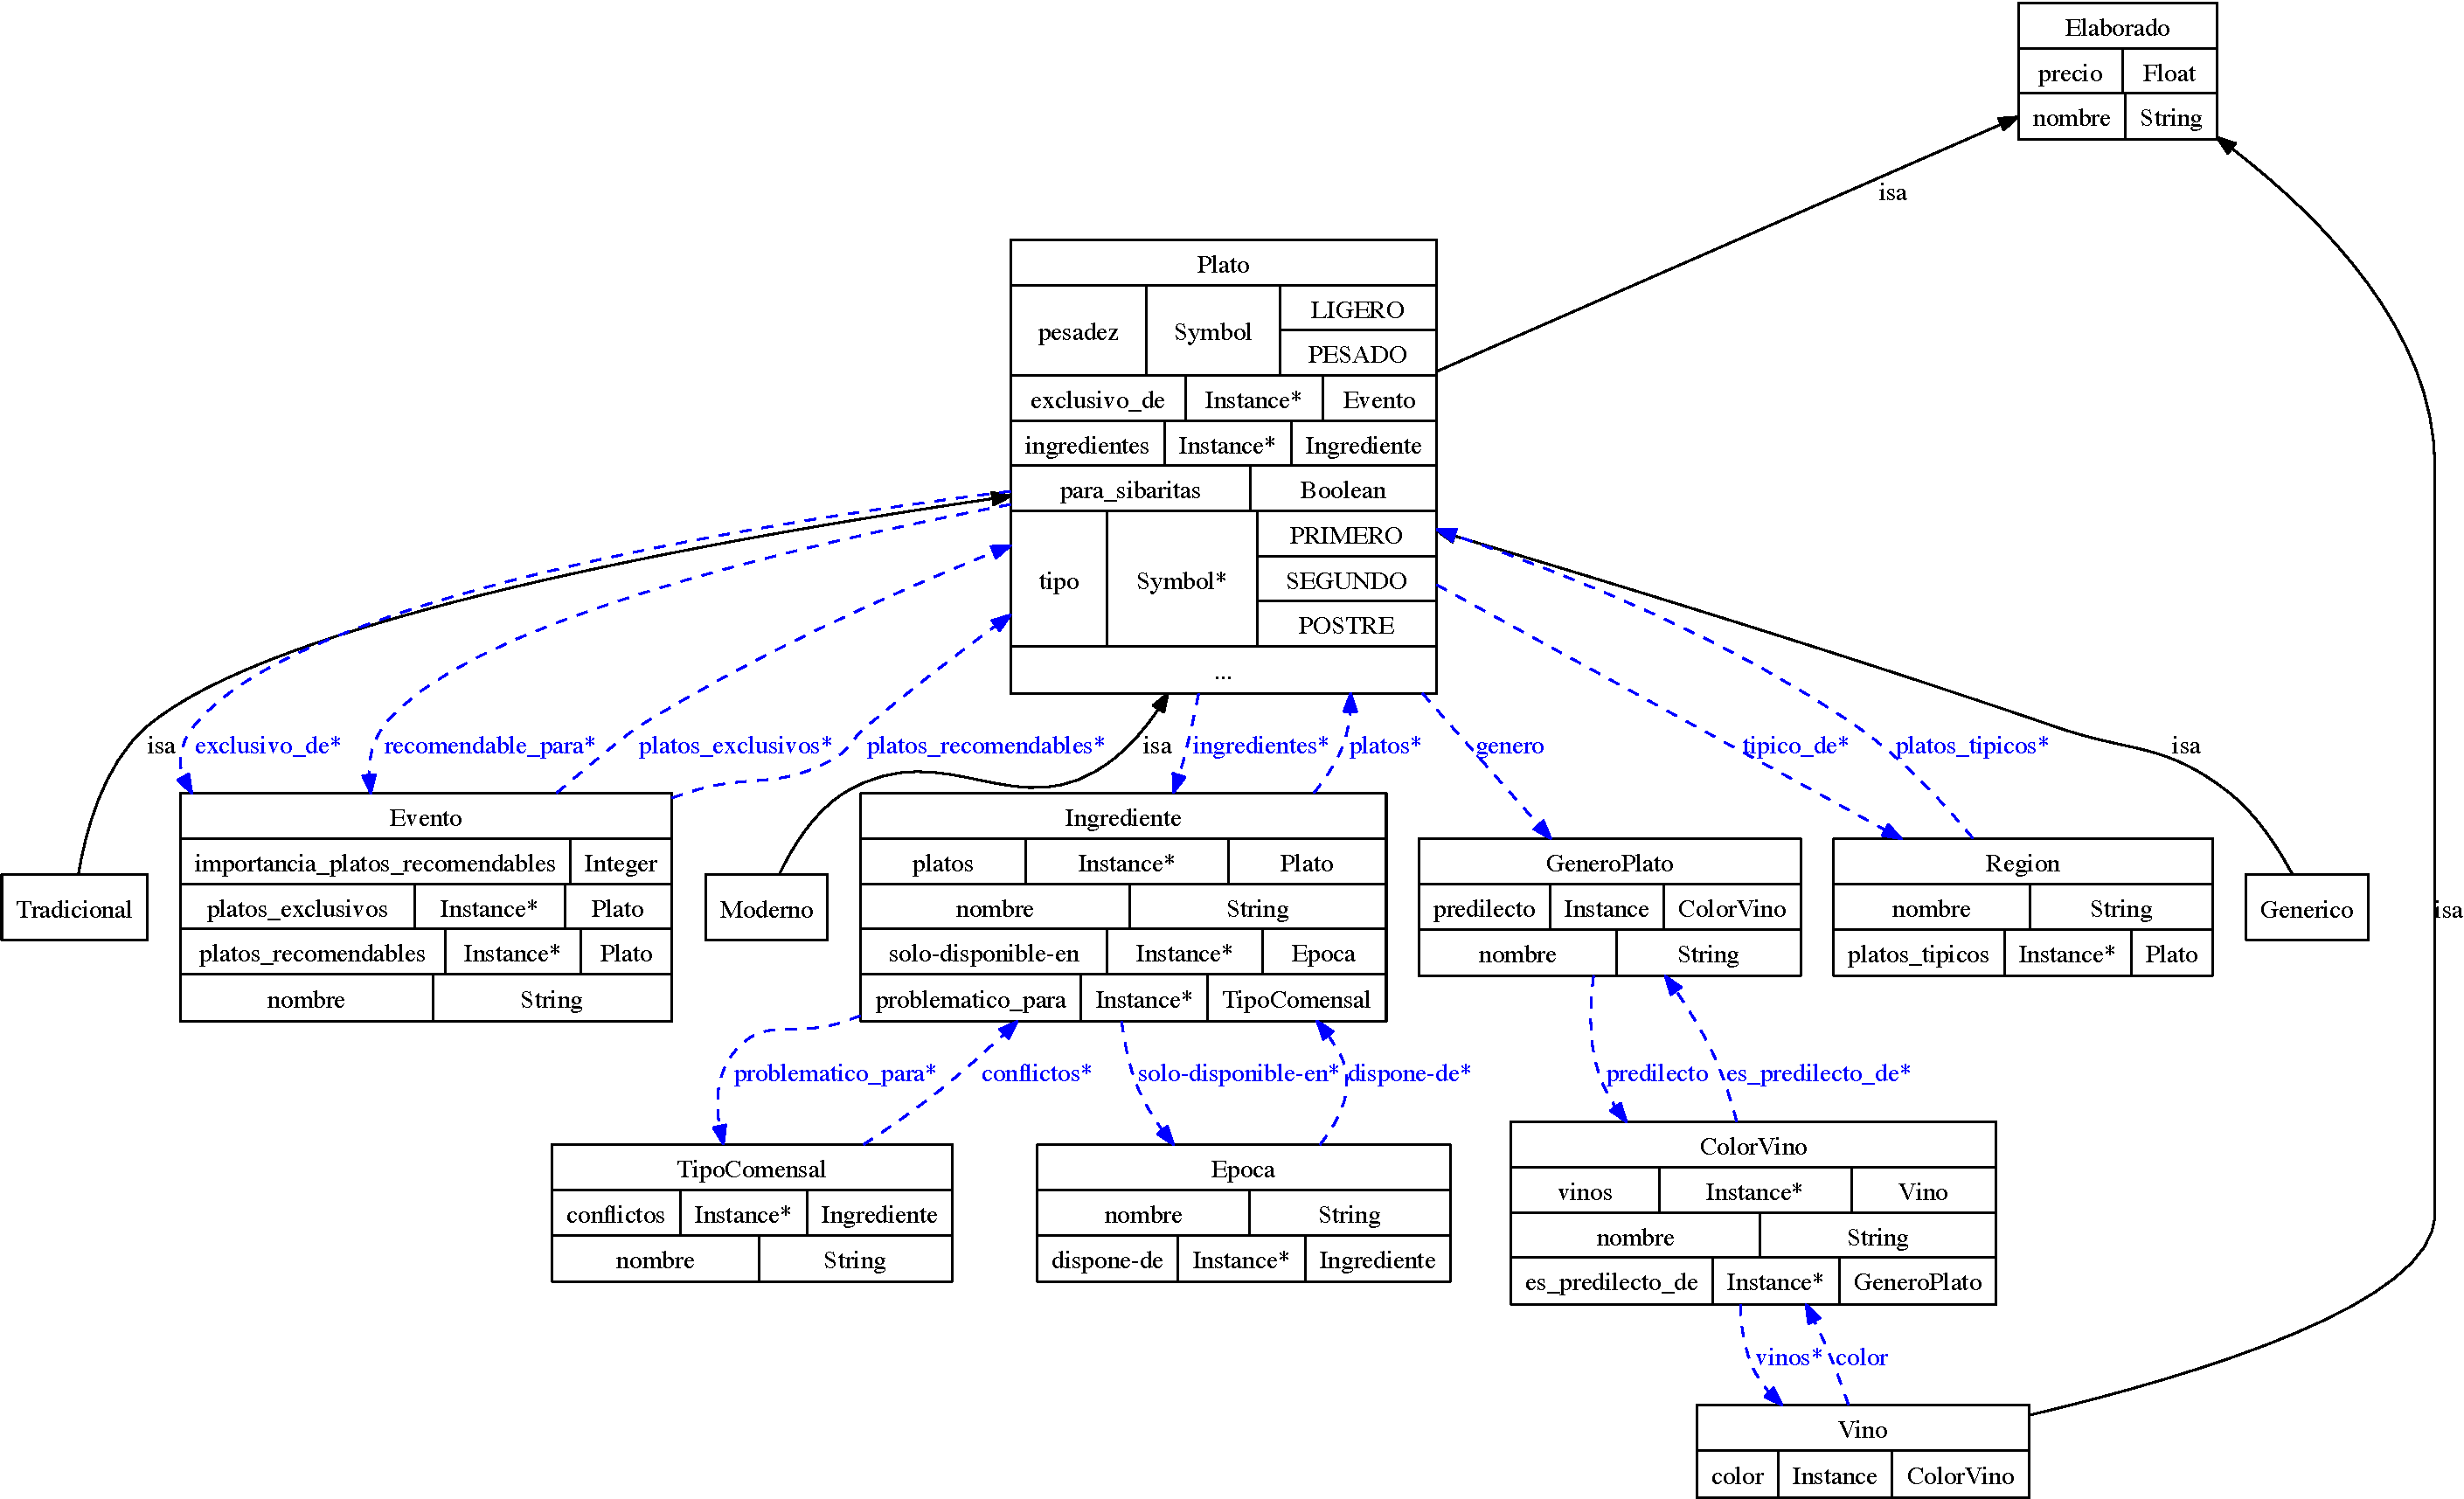
\includegraphics[width=1.2\textwidth]{%
      figures/ontologia}}
  \caption{La ontología final}
\end{figure}

La construcción de la ontología (y de todo el sistema en general) se ha
realizado de manera iterativa, aunque inicialmente no había sido así.

En un principio habíamos construido sistema de clases completo pero incluso más
complejo de lo que ha sido finalmente, sin necesidad. Afortunadamente, esa
versión se perdió y empezamos con una más simple que solamente contenía las
clases elaborado, plato, bebida (que ahora es solamente vino) e ingrediente.

Luego añadimos la clase de tipos de comensal, para poder tener en cuenta
alergias y demás problemas alimenticios. También se añadió la clase época para
poder indicar la disponibilidad de ingredientes.

Inicialmente, los eventos iban a ser unos valores prefijados hasta que vimos
que podríamos sacarle más provecho a todo si eran instancias dentro de la
ontología. Así que creamos la clase evento y asociamos algunos platos como
preferidos en el evento. Para evitar que determinados platos propios de un
evento se recomendaran en otros donde no tuviera sentido (un claro ejemplo son
los pasteles de boda), casi al final hicimos la diferencia entre platos propios
y platos que son recomendables para los eventos.

Ya, más entrados en el proceso de implementación del sistema experto, añadimos
la clase región para poder modelar el origen geográfico/cultural de los
platos. Finalmente, cuando empezamos a tratar con los vinos, y tras considerar
que la bebida en general no tiene sentido para el problema que se nos pide
resolver, eliminamos la clase bebida, dejando solamente una clase para
vinos. Además, creamos la clase que modela el color del vino, que se asoció a
la nueva clase de géneros de plato (sopa, pescado, estofado, aperitivo, etc.)
para poder hacer la recomendación de vinos de manera más sencilla.

Fuera de aquí, también están las ontologías de solución del problema, que
solamente contienen las clases menú y menú abstracto. Más adelante detallaremos
su funcionamiento.

\subsection{Detalle de las clases de la ontología del problema}
\subsubsection{Clase elaborado}
Esta clase está construida para agrupar las características propias de los
productos que se venden con el menú: el nombre y el precio. La idea es que
cualquier cosa que esté en el menú debe ser un producto elaborado.

Es importante notar que la clase es concreta. Esto es así porque el lenguaje
CLIPS así lo precisa para poder hacer \emph{pattern matching}.

\subsubsection{Clase plato y sus subclases}
Esta clase, que originalmente era abstracta, es concreta porque elaborado lo
es.
